\documentclass[12pt]{article}
\usepackage[utf8]{inputenc}
\usepackage[spanish]{babel}
\decimalpoint
\usepackage{amsmath}
\usepackage{caption}
\usepackage{amsthm}
\usepackage{amssymb}
\usepackage{graphicx}
\usepackage[margin=0.9in]{geometry}
\usepackage{fancyhdr}
\usepackage[inline]{enumitem}
\usepackage{float}
\usepackage{cancel}
\usepackage{bigints}
\usepackage{color}
\usepackage{xcolor}
\usepackage{listingsutf8}
\usepackage{algorithm}
\usepackage{tocloft}
\usepackage[none]{hyphenat}
\usepackage{graphicx}
\usepackage{grffile}
\usepackage{tabularx}
\usepackage[nottoc,notlot,notlof]{tocbibind}
\usepackage{times}
\usepackage{color}
\definecolor{gray97}{gray}{.97}
\definecolor{gray75}{gray}{.75}
\definecolor{gray45}{gray}{.45}
\renewcommand{\cftsecleader}{\cftdotfill{\cftdotsep}}
\pagestyle{fancy}
\setlength{\headheight}{15pt} 
\lhead{Práctica 2 - Análisis temporal y notación de orden (Algoritmos de búsqueda)}
\rhead{\thepage}
\lfoot{ESCOM-IPN}
\renewcommand{\footrulewidth}{0.5pt}
\setlength{\parskip}{0.5em}
\newcommand{\ve}[1]{\overrightarrow{#1}}
\newcommand{\abs}[1]{\left\lvert #1 \right\lvert}
\date{26 de febrero de 2017}
\title{Pruebas a posteriori}
\author{Reporte 1}

\definecolor{pblue}{rgb}{0.13,0.13,1}
\definecolor{pgreen}{rgb}{0,0.5,0}
\definecolor{pred}{rgb}{0.9,0,0}
\definecolor{pgrey}{rgb}{0.46,0.45,0.48}
\lstset{tabsize=1}

\usepackage{listings}
\lstset{ frame=Ltb,
framerule=0pt,
aboveskip=0.5cm,
framextopmargin=3pt,
framexbottommargin=3pt,
framexleftmargin=0.4cm,
framesep=0pt,
rulesep=.4pt,
backgroundcolor=\color{gray97},
rulesepcolor=\color{black},
%
stringstyle=\ttfamily,
showstringspaces = false,
basicstyle=\small\ttfamily,
commentstyle=\color{gray45},
keywordstyle=\bfseries,
%
numbers=left,
numbersep=15pt,
numberstyle=\tiny,
numberfirstline = false,
breaklines=true,
}

% minimizar fragmentado de listados
\lstnewenvironment{listing}[1][]
{\lstset{#1}\pagebreak[0]}{\pagebreak[0]}

\lstdefinestyle{consola}
{basicstyle=\scriptsize\bf\ttfamily,
backgroundcolor=\color{gray75},
}

\lstdefinestyle{Java}
{language=Java,
}

%%%%%%%%%%%%%%%%%%%%%

\lstdefinestyle{customc}{
  belowcaptionskip=1\baselineskip,
  breaklines=true,
  frame=L,
  xleftmargin=\parindent,
  language=C,
  showstringspaces=false,
  basicstyle=\footnotesize\ttfamily,
  keywordstyle=\bfseries\color{green!40!black},
  commentstyle=\itshape\color{purple!40!black},
  identifierstyle=\color{blue},
  stringstyle=\color{orange},
}

\lstdefinestyle{customasm}{
  belowcaptionskip=1\baselineskip,
  frame=L,
  xleftmargin=\parindent,
  language=[x86masm]Assembler,
  basicstyle=\footnotesize\ttfamily,
  commentstyle=\itshape\color{purple!40!black},
}

\lstset{escapechar=@,style=customc}


    % =====  CODE EDITOR =========
    \lstdefinestyle{CompilandoStyle} {                              %This is Code Style
        backgroundcolor=\color{BlueGrey800MD},                      %Background Color  
        basicstyle=\tiny\color{white},                              %Font color
        commentstyle=\color{BlueGrey100MD},                         %Comment color
        stringstyle=\color{TealMD},                                 %String color
        keywordstyle=\color{Green100MD},                            %keywords color
        numberstyle=\tiny\color{TealMD},                            %Size of a number
        frame=shadowbox,                                            %Adds a frame around the code
        breakatwhitespace=true,                                     %Style                       
        breaklines=true,                                            %Style                   
        keepspaces=true,                                            %Style                   
        numbers=left,                                               %Style                   
        numbersep=10pt,                                             %Style 
        xleftmargin=\parindent,                                     %Style 
        tabsize=4                                                   %Style 
    }
 
    \lstset{style=CompilandoStyle}                                  %Use this style

    \usepackage{minted} % Paquete que permite citar codigo
    \usemintedstyle{borland} % Aqui se define el colorscheme para minted
    \setminted{
        fontsize = \scriptsize, % Ajusta el codigo a la hoja
        baselinestretch = 1,
        linenos, % set numbers
        breaklines=true, % Hace un salto de linea automatico en caso de que se llege al final de la line
        tabsize=3 
    }

%Permite crear columnas en el documento
\usepackage{multicol} 
\usepackage{color}
\usepackage{comment}
\newcommand{\tabitem}{~~\llap{\textbullet}~~}
\newcommand{\subtabitem}{~~~~\llap{\textbullet}~~}

\bibliographystyle{IEEEtran}
\begin{document}
		\begin{titlepage}
			\begin{center}
				
				% Upper part of the page. The '~' is needed because \\
				% only works if a paragraph has started.
				
				\noindent
				\begin{minipage}{0.5\textwidth}
					\begin{flushleft} \large
						\includegraphics[width=0.3\textwidth]{../ipn.png}
					\end{flushleft}
				\end{minipage}%
				\begin{minipage}{0.55\textwidth}
					\begin{flushright} \large
						\includegraphics[width=0.7\textwidth]{../escom.png}
					\end{flushright}
				\end{minipage}
				
				\textsc{\LARGE Instituto Politécnico Nacional}\\[0.5cm]
				
				\textsc{\Large Escuela Superior de Cómputo}\\[1cm]
				
				% Title
				
				{ \huge Práctica 2 - Análisis temporal y notación de orden (Algoritmos de búsqueda)\\[1cm] }
				
				{ \Large Unidad de aprendizaje: Análisis de Algoritmos} \\[1cm]
				
				{ \Large Grupo: 3CM3} \\[1cm]
				
				\noindent
				\begin{minipage}{0.5\textwidth}
					\begin{flushleft} \large
						\emph{Alumnos(a): "La naranja mecánica"}\\
						
						\begin{tabular}{ll}
					     Nicolás Sayago Abigail\\
					     Parra Garcilazo Cinthya Dolores\\
					     Ramos Díaz Enrique \\
					
					\end{tabular}
					\end{flushleft}
				\end{minipage}%
				\begin{minipage}{0.5\textwidth}
					\begin{flushright} \large
						\emph{Profesor(a): Edgardo Adrián Franco Martínez} \\
						  \\
					\end{flushright}
				\end{minipage}
				
					\begin{minipage}{0.5\textwidth}
					\begin{center} \large
						\includegraphics[width=0.8\textwidth]{../xd.jpg}
						\caption*{"La Naranja Mecánica"}
					\end{center}
				\end{minipage}

				\vfill
				
				% Bottom of the page
				{\large 10 de Octubre 2018}
			\end{center}
		\end{titlepage}
	
	\tableofcontents
	\newpage
	% /////////////////////////////////////////////////////////
	%			PLANTEAMIENTO DEL PROBLEMA
	% ////////////////////////////////////////////////////////
	\section{Planteamiento del problema}
	Existen diversos métodos de búsqueda numérica, en este documento se analizaran 3, se observará y comparará el comportamiento de cada uno, para determinar el mejor de todos.
    
    Se tomaran resultados experimentales en una plataforma determinada para determinar la complejidad temporal y su orden de complejidad (cota O mayúscula) de los siguientes algoritmos: Búsqueda Lineal, Búsqueda Binaria y Árbol de Búsqueda Binario.
    
    Además, se analizará la efectividad y velocidad de la implementación de éstos algoritmos con ejecución de hilos simultáneos, para determinar si vale o no la pena al momento de ahorrar recursos de nuestra computadora para tamaños de problema muy grandes.

	
	% /////////////////////////////////////////////////////////
	%			PLATAFORMA EXPERIMENTAL
	% ////////////////////////////////////////////////////////
    \section{Plataforma Experimental}
	
	    \textbf{Especificaciones de Hardware:}
	    \begin{itemize}
	        \item CPU: Intel Core-i5 6500 3.2 GHz
	        \item Memoria: RAM DDR4 5.9 GB 2133 MHz
	    \end{itemize}
    
	    \textbf{Compilador:} GCC version 7.3.0 desde la Terminal
	    
	    \textbf{Sistema Operativo:} Linux Ubuntu 18.04.1 LTS x64 

	% /////////////////////////////////////////////////////////
	%			ACTIVIDADES Y PRUEBAS
	% ////////////////////////////////////////////////////////
	
	\section{Actividades y Pruebas}
	
		% ----------------------------------------------------
		% 					BUSQUEDA LINEAL
		% ----------------------------------------------------
	    \subsection{Búsqueda Lineal}
	        \subsubsection{Análisis teórico a priori}
	        \begin{figure}[H]
			    	   \centering
			    	   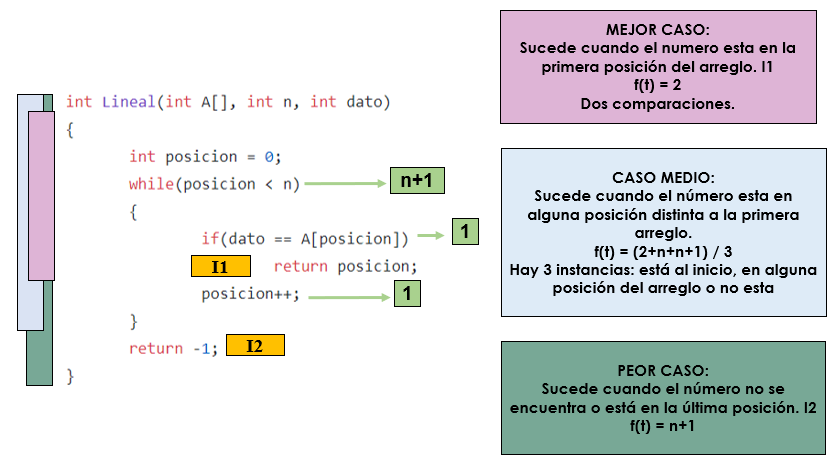
\includegraphics[width=0.9\textwidth]{images/cotas/lineal_analisis.PNG}
			    \end{figure}
	        
	        \subsubsection{Ejecución del algoritmo}
            	\begin{figure}[H]
                	   \centering
                	   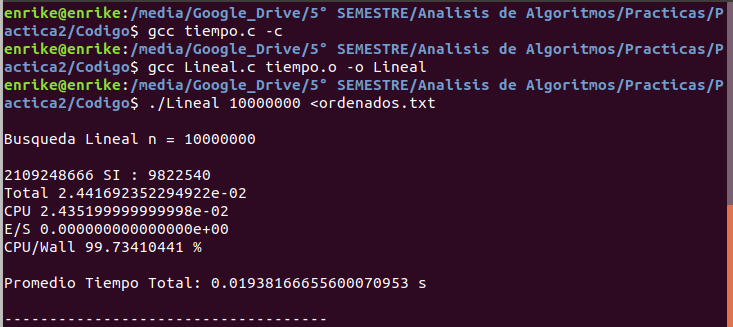
\includegraphics[width=0.9\textwidth]{images/pruebas/lineal.png}
                \end{figure}
	        
	        \subsubsection{Análisis temporal promedio}
            	\begin{figure}[H]
            	    \centering
                	   \includegraphics[width=0.95\textwidth]{images/tablas/Lineal.JPG}
                \end{figure}
        	
        	\subsubsection{Gráfica de comportamiento}
            	\begin{figure}[H]
            	    \centering
                	   \includegraphics[width=0.9\textwidth]{images/graficas/lineal.PNG}
                \end{figure}
    
        	\subsubsection{Aproximación Polinomial}
        	\begin{figure}[H]
    			  \centering
    			 \includegraphics[width=0.85\textwidth]{images/polinomios/lineal.PNG}
    			    	   \caption*{\textbf{Grado 1: $0.000236308 + 1.75588\times10^{-9} x$}}
    			  \end{figure}

        	\subsubsection{Tiempo por cada operación básica}
        	Tomamos la función de complejidad temporal del peor caso. \textcolor{blue}{ Peor Caso $f_{tpc}(n) = n+1$}
    			
    			Luego, tomamos el polinomio obtenido en la aproximación polinomial en función de n: 
    			
    			$P(n) = 0.000236308 + 1.75588\times10^{-9} x$
    			
    			Utilizaremos un tamaño de problema n = 10000000 para el cálculo.
    			
    			Calculamos el número de operaciones para un tamaño de problema n con la función de complejidad temporal del peor caso:
    			
    			$$f_{tpc}(10000000) = 10000000+1 = 10000001~operaciones$$
    			
    			Ahora, calculamos el tiempo en segundos con el polinomio:
    			
    			$$P(10000000) = 0.0177951~segundos$$
    			
    			El tiempo en que tarda cada operación básica es:
    			
    			$$Tiempo~x~op.~básica = \frac{0.0177951}{10000001} =1.7795\times10^{-9}~segundos$$
    
        	\subsubsection{Evaluación de tamaños de problema n's}
        	Para n = 50000000
    			
                $P(50000000) = 0.0880303~ segundos$
    
    			Para n = 100000000
    			
    			$P(100000000) = 0.175824~ segundos$
    			
    			Para n = 500000000
    			
    			$P(500000000) = 0.878176~ segundos$
    			
    			Para n = 1000000000
    			
    			$P(1000000000) = 1.75612~ segundos$
    			
    			Para n = 5000000000
    			
    			$P(5000000000) = 8.77964~ segundos$
    
    		\subsubsection{Cota O mayúscula del algoritmo}

			\begin{figure}[H]
			    	   \centering
			    	   \includegraphics[width=0.9\textwidth]{images/cotas/Lineal.PNG}
			    \end{figure}
			    
			    \subsubsection{Cota O mayúscula del polinomio}
			    Al tratarse de un polinomio de grado 1, su cota de complejidad O sera $O(n)$.
			    

    		  
	
\newpage

		% ----------------------------------------------------
		% 					BUSQUEDA LINEAL HILOS
		% ----------------------------------------------------

		\subsection{Búsqueda Lineal (Hilos)}
			
			\subsubsection{Funcionamiento}
			Según la cantidad n de hilos que se envíen como parámetro al ejecutar el programa, estos dividirán el arreglo en n partes. En cada una de ellas se ejecutará de manera simultanea el algoritmo de búsqueda lineal indicado anteriormente; va buscando posición por posición el número en el pedazo del arreglo. Con ayuda del número de hilos podemos establecer los rangos, con un índice (posición del arreglo) de inicio y otro de fin, que le corresponderán a cada hilo en su ejecución.
			
			\subsubsection{Ejecución del algoritmo}
				\begin{figure}[H]
			    	   \centering
			    	   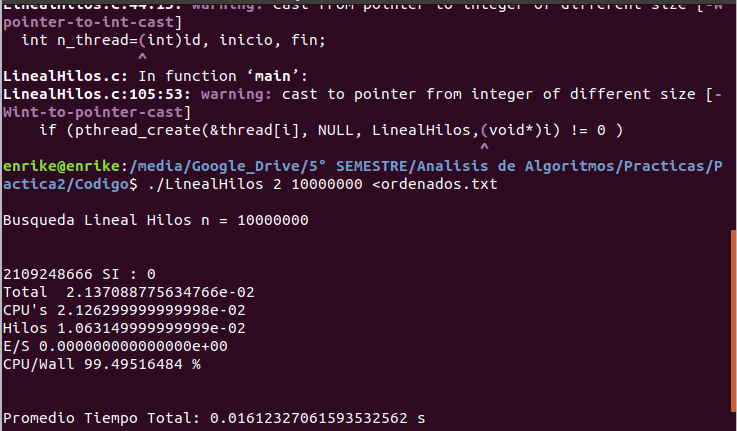
\includegraphics[width=0.8\textwidth]{images/pruebas/linealhilos.png}
			    \end{figure}
			
			\subsubsection{Análisis temporal promedio}
				\begin{figure}[H]
				    \centering
			    	   \includegraphics[width=0.95\textwidth]{images/tablas/LinealHilos.JPG}
			    \end{figure}
			
			\subsubsection{Gráfica de comportamiento}
				\begin{figure}[H]
				    \centering
			    	   \includegraphics[width=0.9\textwidth]{images/graficas/LinealHilosGrafica.JPG}
			    \end{figure}
			
			\subsubsection{Aproximación Polinomial}
			\begin{figure}[H]
    			  \centering
    			 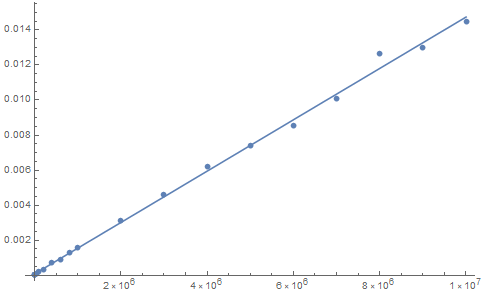
\includegraphics[width=0.85\textwidth]{images/polinomios/linealhilos.PNG}
    			    	   \caption*{\textbf{Grado 1: $0.0000858628 + 1.46546*10^{-9} x$}}
    			  \end{figure}
			
			\newpage
			\subsubsection{Evaluación de tamaños de problema n's}
			Para n = 50000000
    			
                $P(50000000) = 0.0733589~ segundos$
    
    			Para n = 100000000
    			
    			$P(100000000) = 0.146632~ segundos$
    			
    			Para n = 500000000
    			
    			$P(500000000) = 0.732816~ segundos$
    			
    			Para n = 1000000000
    			
    			$P(1000000000) = 1.46555~ segundos$
    			
    			Para n = 5000000000
    			
    			$P(5000000000) = 7.32739~ segundos$
			
		\subsubsection{Cotas O mayúscula del polinomio}
		Al tratarse de un polinomio de grado 1, su cota de complejidad O sera $O(n)$.
			
\newpage

		% ----------------------------------------------------
		% 					BUSQUEDA BINARIA
		% ----------------------------------------------------	
	
		\subsection{Búsqueda Binaria}
			
			\subsubsection{Análisis teórico a priori}
			\begin{figure}[H]
			    	   \centering
			    	   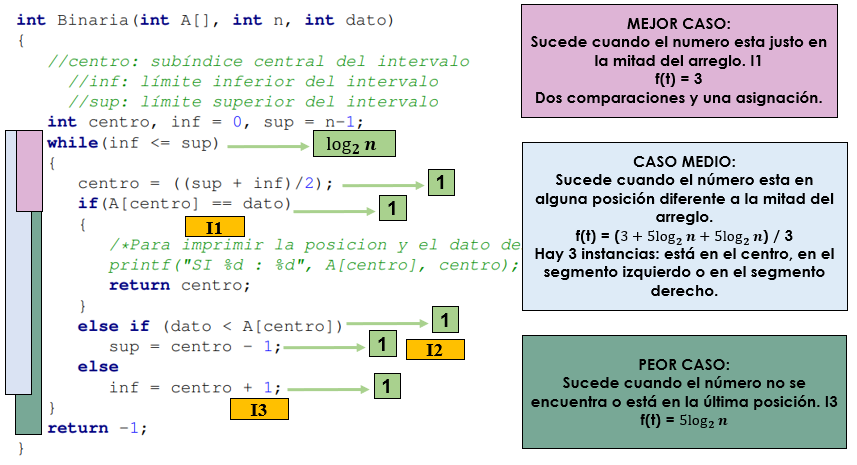
\includegraphics[width=0.9\textwidth]{images/cotas/binaria_analisis.PNG}
			    \end{figure}
			
			\subsubsection{Ejecución del algoritmo}
				\begin{figure}[H]
			    	   \centering
			    	   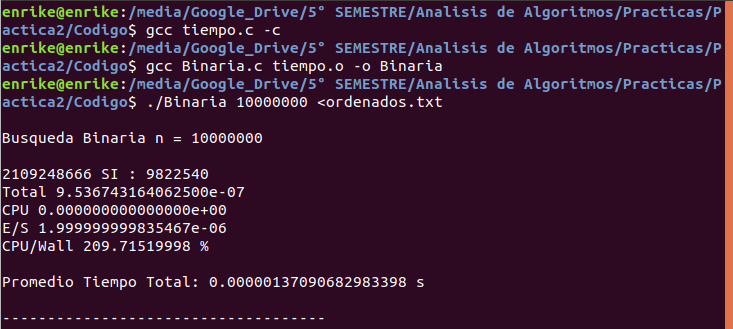
\includegraphics[width=0.9\textwidth]{images/pruebas/binaria.png}
			    \end{figure}
			
			\subsubsection{Análisis temporal promedio}
				\begin{figure}[H]
			    	   \centering
			    	   \includegraphics[width=0.95\textwidth]{images/tablas/binaria.PNG}
			    \end{figure}
			
			\subsubsection{Gráfica de comportamiento}
				\begin{figure}[H]
			    	   \centering
			    	   \includegraphics[width=0.9\textwidth]{images/graficas/binaria.PNG}
			    \end{figure}
			
			\subsubsection{Aproximación Polinomial}
				\begin{figure}[H]
			    	   \centering
			    	   \includegraphics[width=0.85\textwidth]{images/polinomios/binaria.PNG}
			    	   \caption*{\textbf{Grado 5: $7.20374\times10^{-7} + 2.42704\times10^{-13} x - 6.58073\times10^{-20} x^2 + 
			            1.16759\times10^{-26} x^3 - 1.10283\times10^{-33} x^4 + 4.15462\times10^{-41} x^5$}}
			    \end{figure}
			
			\subsubsection{Tiempo por cada operación básica}
    			Tomamos la función de complejidad temporal del peor caso. \textcolor{blue}{ Peor Caso $f_{tpc}(n) = 5log_2n$}
    			
    			Luego, tomamos el polinomio obtenido en la aproximación polinomial en función de n: $P(n) = 7.20374\times10^{-7} + 2.42704\times10^{-13} n - 6.58073\times10^{-20} n^2 + 
    			1.16759\times10^{-26} n^3 - 1.10283\times10^{-33} n^4 + 4.15462\times10^{-41} n^5$
    			
    			Utilizaremos un tamaño de problema n = 10000000 para el cálculo.
    			
    			Calculamos el número de operaciones para un tamaño de problema n con la funcion de complejidad temporal del peor caso:
    			
    			$$f_{tpc}(10000000) = 5log_210000000 = 116~operaciones$$
    			
    			Ahora, calculamos el tiempo en segundos con el polinomio:
    			
    			$$P(10000000) = 1.3689\times10^{-6}~ segundos$$
    			
    			El tiempo en que tarda cada operación básica es:
    			
    			$$Tiempo~x~op.~básica = \frac{1.3689\times10^{-6}}{116} = 1.18\times10^{-8}~segundos$$
    			
    			\subsubsection{Evaluación de tamaños de problema n's}
    			Para n = 50000000
    			
                $P(50000000) = 0.00739832~ segundos$
    
    			Para n = 100000000
    			
    			$P(100000000) = 0.316222~ segundos$
    			
    			Para n = 500000000
    			
    			$P(500000000) = 1230.84~ segundos$
    			
    			Para n = 1000000000
    			
    			$P(1000000000) = 40455~ segundos$
    			
    			Para n = 5000000000
    			
    			$P(5000000000) = 1.29144\times10^{8}~ segundos$
    			
			\subsubsection{Cota O mayúscula del algoritmo}

		    	\begin{figure}[H]
			    	   \centering
			    	   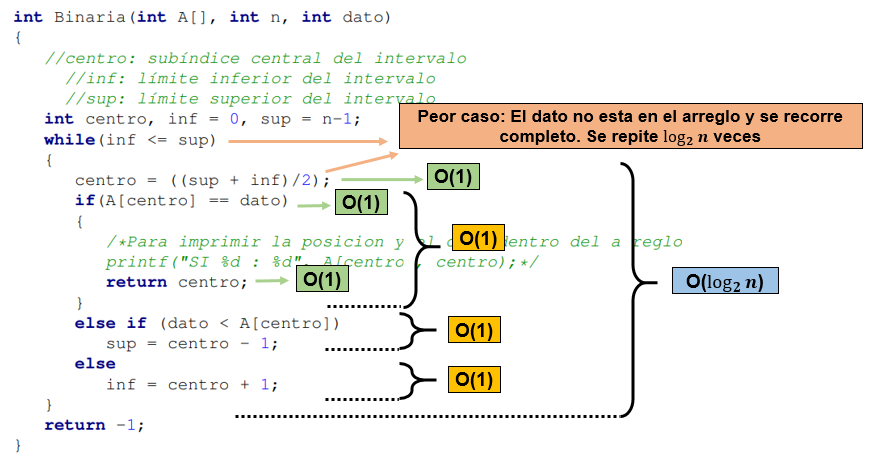
\includegraphics[width=0.9\textwidth]{images/cotas/Binaria.PNG}
			    \end{figure}
			    
			    \subsubsection{Cota O mayúscula del polinomio}
			    Al tratarse de un polinomio de grado 5, su cota de complejidad O sera $O(n^5)$.
				
\newpage
		% ----------------------------------------------------
		% 					BUSQUEDA BINARIA HILOS
		% ----------------------------------------------------

		\subsection{Búsqueda Binaria (Hilos)}
			
			\subsubsection{Funcionamiento}
			Según la cantidad n de hilos que se envíen como parámetro al ejecutar el programa, estos dividirán el arreglo en n partes. En cada una de ellas se ejecutará de manera simultanea el algoritmo de búsqueda binaria indicado anteriormente; se divide en dos cada pedazo del arreglo y se recorre hasta encontrar el número, ya sea a la izquierda o derecha. Con ayuda del número de hilos podemos establecer los rangos, con un índice (posición del arreglo) de inicio y otro de fin, que le corresponderán a cada hilo en su ejecución.
			
			\subsubsection{Ejecución del algoritmo}
				\begin{figure}[H]
			    	   \centering
			    	   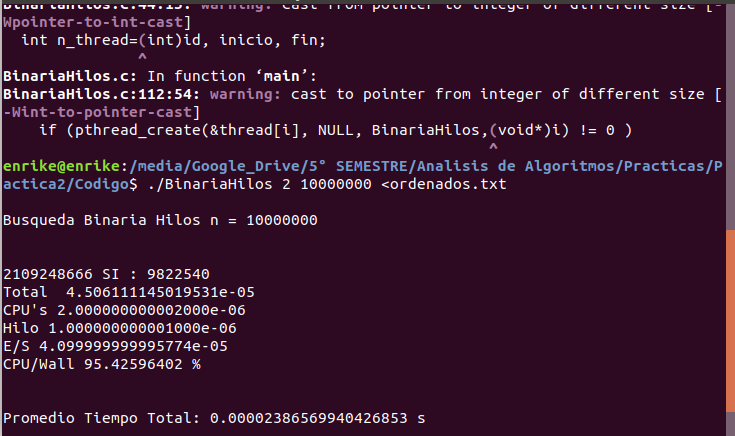
\includegraphics[width=0.9\textwidth]{images/pruebas/binariahilos.png}
			    \end{figure}
			
			\subsubsection{Análisis temporal promedio}
				\begin{figure}[H]
			    	   \centering
			    	   \includegraphics[width=0.95\textwidth]{images/tablas/binariahilos.PNG}
			    \end{figure}
			
			\subsubsection{Gráfica de comportamiento}
				\begin{figure}[H]
			    	   \centering
			    	   \includegraphics[width=0.9\textwidth]{images/graficas/binariahilos.PNG}
			    \end{figure}
			
			\subsubsection{Aproximación Polinomial}
				\begin{figure}[H]
			    	   \centering
			    	   \includegraphics[width=0.85\textwidth]{images/polinomios/binariahilos.PNG}
			    	   \caption*{\textbf{Grado 5: $0.0000211462 + 6.03491\times10^{-12} x - 5.65412\times10^{-18} x^2 + 
                        1.76786\times10^{-24} x^3 - 2.1856\times10^{-31} x^4 + 9.28242\times10^{-39} x^5$}}
			    \end{figure}
			
			\subsubsection{Evaluación de tamaños de problema n's}
    			Para n = 50000000
    			
                $P(50000000) = 1.74193~ segundos$
    
    			Para n = 100000000
    			
    			$P(100000000) = 72.6801\times10^{6}~ segundos$
    			
    			Para n = 500000000
    			
    			$P(500000000) = 276635~ segundos$
    			
    			Para n = 1000000000
    			
    			$P(1000000000) = 9.06562\times10^6~ segundos$
    			
    			Para n = 5000000000
    			
    			$P(5000000000) = 2.88712\times10^{10}~ segundos$

			\subsubsection{Cota O mayúscula del polinomio}
			    Al tratarse de un polinomio de grado 5, su cota de complejidad O sera \textbf{$O(n^5)$}.
		
\newpage

		% ----------------------------------------------------
		% 				ARBOL DE BUSQUEDA BINARIA
		% ----------------------------------------------------

		\subsection{Árbol de Búsqueda Binaria}
			
			\subsubsection{Análisis teórico a priori}
				\begin{figure}[H]
			    	   \centering
			    	   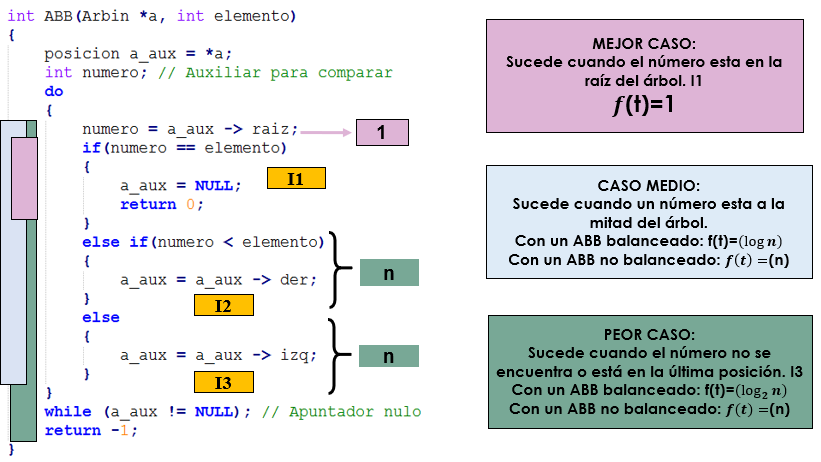
\includegraphics[width=0.9\textwidth]{images/cotas/ABB_Analisis.PNG}
			    \end{figure}
			
			\subsubsection{¿Por qué no usar hilos?}
			    Por que no se puede hacer la segmentación de manera correcta como en los demás algoritmos. La segmentación y recorrido del árbol en diferentes rangos va desechando aquellos nodos en los que no se encuentra el número a buscar, por lo que solo causaría que en muchos de ellos no buscaran nada, lo cual seria un gasto de recursos al crear los hilos.
			
			\subsubsection{Ejecución del algoritmo}
				\begin{figure}[H]
			    	   \centering
			    	   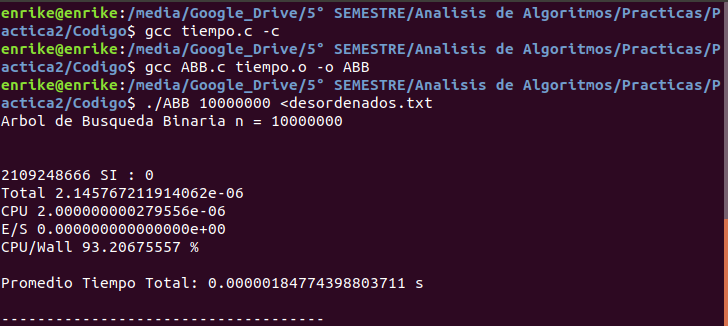
\includegraphics[width=0.9\textwidth]{images/pruebas/abb.png}
			    \end{figure}

			\subsubsection{Análisis temporal promedio}
				\begin{figure}[H]
			    	   \centering
			    	   \includegraphics[width=0.95\textwidth]{images/tablas/ABB.PNG}
			    \end{figure}
			
			\subsubsection{Gráfica de comportamiento}
				\begin{figure}[H]
			    	   \centering
			    	   \includegraphics[width=0.9\textwidth]{images/graficas/ABB.PNG}
			    \end{figure}
			
			\subsubsection{Aproximación Polinomial}
    			\begin{figure}[H]
    			  \centering
    			 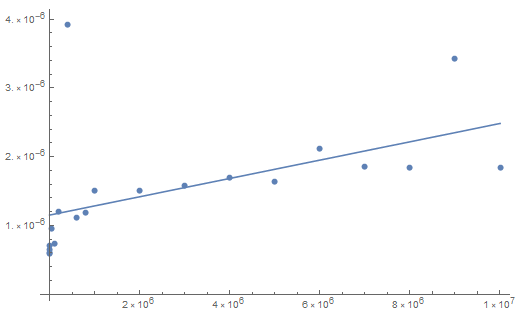
\includegraphics[width=0.85\textwidth]{images/polinomios/abb.PNG}
    			    	   \caption*{\textbf{Grado 1: $1.15287\times10^{-6} + 1.33212\times10^{-13} x$}}
    			  \end{figure}


			\subsubsection{Tiempo por cada operación básica}
			    Tomamos la función de complejidad temporal del peor caso. \textcolor{blue}{ Peor Caso $f_{tpc}(n) = n$}
			
    			Luego, tomamos el polinomio obtenido en la aproximación polinomial en función de n: $P(n) = 1.15287\times10^{-6} + 1.33212\times10^{-13} x$
    			
    			Utilizaremos un tamaño de problema n = 10000000 para el cálculo.
    			
    			Calculamos el número de operaciones para un tamaño de problema n con la función de complejidad temporal del peor caso:
    			
    			$$f_{tpc}(10000000) = 10000000 = 10000000 ~operaciones$$
    			
    			Ahora, calculamos el tiempo en segundos con el polinomio:
    			
    			$$P(10000000) = 2.48499\times10^{-6}~ segundos$$
    			
    			El tiempo en que tarda cada operación básica es:
    			
    			$$Tiempo~x~op.~básica = \frac{2.48499\times10^{-6}}{10000000} = 2.48499\times10^{-13}~segundos$$
\newpage
			\subsubsection{Evaluación de tamaños de problema n's}
    			Para n = 50000000
    			
                $P(50000000) = 7.81347\times10^{-6}~ segundos$
    
    			Para n = 100000000
    			
    			$P(100000000) = 0.0000144741~ segundos$
    			
    			Para n = 500000000
    			
    			$P(500000000) = 0.0000677589~ segundos$
    			
    			Para n = 1000000000
    			
    			$P(1000000000) = 0.000134365~ segundos$
    			
    			Para n = 5000000000
    			
    			$P(5000000000) = 0.000667213~ segundos$
    		
			\subsubsection{Cota O mayúscula del algoritmo}
			    \begin{figure}[H]
			    	   \centering
			    	   \includegraphics[width=0.9\textwidth]{images/cotas/ABB.PNG}
			    \end{figure}
			    
			\subsubsection{Cota O mayúscula del polinomio}
			    Al tratarse de un polinomio de grado 1, su cota de complejidad O sera \textbf{$O(n)$}.
			
		% ----------------------------------------------------
		% 					COMPARATIVAS
		% ----------------------------------------------------
		\newpage	
			\subsection{Comparativa gráfica de comportamiento (Tiempo Real promedio)}
			
			\begin{figure}[H]
			    	   \centering
			    	   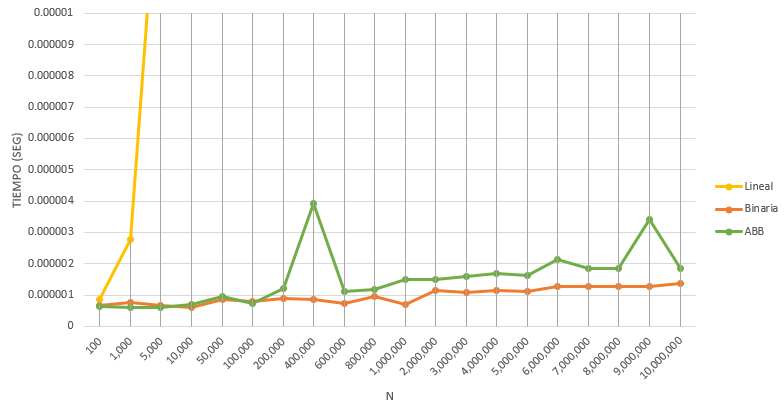
\includegraphics[width=0.9\textwidth]{images/graficas/comp1.PNG}
			    \end{figure}
			    
			    \begin{figure}[H]
			    	   \centering
			    	   \includegraphics[width=0.9\textwidth]{images/graficas/comp2.PNG}
			    \end{figure}
			    \newpage
			\subsection{Comparativa gráfica de comportamiento con Hilos (Tiempo Real promedio)}
			
			    \begin{figure}[H]
			    	   \centering
			    	   \includegraphics[width=0.9\textwidth]{images/graficas/comphilos.PNG}
			    \end{figure}
			
			\subsection{Comparativa de aproximaciones polinomiales}
			\begin{figure}[H]
			    	   \centering
			    	   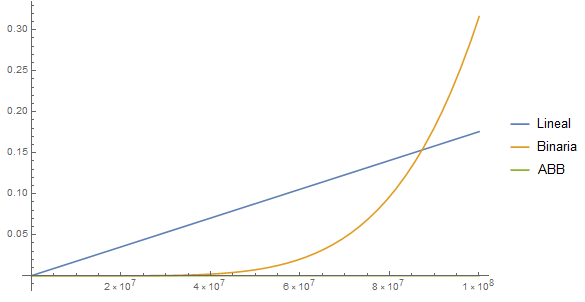
\includegraphics[width=0.9\textwidth]{images/polinomios/comp.PNG}
			    \end{figure}
			    
			    \begin{figure}[H]
			    	   \centering
			    	   \includegraphics[width=0.9\textwidth]{images/polinomios/comp2.PNG}
			    \end{figure}
			
			\subsection{Comparativa de aproximaciones polinomiales (Hilos)}
			\begin{figure}[H]
			    	   \centering
			    	   \includegraphics[width=0.9\textwidth]{images/polinomios/comphilos.PNG}
			    \end{figure}
			
\newpage

		% ----------------------------------------------------
		% 					CUESTIONARIO
		% ----------------------------------------------------

		\subsection{Cuestionario}
		\begin{enumerate}
			        \item ¿Cuál de los 3 algoritmos es más fácil de implementar?\\
			        \textbf{El algoritmo de Búsqueda Lineal, ya que las operaciones que utiliza son menores en comparación con los otros algoritmos.}
			        
			        \item ¿Cuál de los 3 algoritmos es más difícil de implementar?\\
			        \textbf{Podría considerase que el algoritmo del Árbol de Búsqueda Binaria fue el más complejo debido al uso de apuntadores que se realizó, los otros dos no hacen uso de éstos.}
			        
			        \item ¿Cuál de los 3 algoritmos es el más difícil de implementar en su variante con hilos?\\
			        \textbf{El algoritmo  de Búsqueda Binaria, pues primero fue necesario identificar en que sección del código se debía de colocar el algoritmo. Además, había que tomar en cuenta el inicio y el fin de cada hilo, y adecuarlo a las variables de control.}
			        
			        \item ¿Cuál de los 3 algoritmos en su variante con hilos resultó ser más rápido?\\
			        \textbf{El de Búsqueda Lineal, ya que se repartió el trabajo de recorrido y comparación posición por posición entre varios hilos simultáneos.}
			        
			        \item ¿Cuál algoritmo tiene menor complejidad temporal?\\
	                \textbf{El de Búsqueda Binaria.}
			        
			        \item ¿Cuál algoritmo tiene mayor complejidad temporal?\\
			        \textbf{El Árbol de Búsqueda Binaria, teniendo en cuenta que no este balanceado, y la Búsqueda Lineal.}
			        \item ¿El comportamiento experimental de los algoritmos era el esperado?¿Por qué?\\
			        \textbf{En la implementación normal de éstos sí. En cambio, en su implementación con hilos sólo hubo mejora en la Búsqueda Lineal, pues en la Binaria el tiempo incluso aumento. Estos es debido a que se utiliza tiempo para crear los hilos, establecer los rangos del arreglo, inicializarlos y esperar a que terminen. Esto significa un uso de recursos innecesario.}
			        
			        \item ¿Sus resultados experimentales difieren mucho de los análisis teóricos que se analizaron? ¿A que se debe?\\
			        \textbf{A grandes rasgos no. Ambos análisis se encuentran dentro de la misma cota de complejidad. En algunos tamaños de problema existen tiempos muy altos o muy pequeños que no siguen el comportamiento esperado del algoritmo.}
			        
			        \item ¿Los resultados experimentales de las implementaciones con hilos de los algoritmos realmente tardaron F(t)/#hilos de su implementación sin hilos?\\
			        \textbf{Sí, pues se hicieron pruebas experimentales en las implementaciones con hilos de los algoritmos creando un único hilo, para comparar los resultados con los de su implementación sin hilos, y efectivamente los tiempos coinciden.}
			        
			        \item ¿Cuál es el \% de mejora que tiene cada uno de los algoritmos en su variante con hilos?¿Es lo que esperabas?¿Por qué?\\
			        \textbf{Para la Búsqueda Lineal, utilizando dos hilos, los tiempos reales promedio mejoraron en un 18.65\% en promedio con respecto a los de la implementación sin hilos.}
			        
			        \textbf{En cambio, para la Búsqueda Binaria, utilizando dos hilos, los tiempos reales promedio empeoraron en un 94.64\% en promedio con respecto a los de la implementación sin hilos.}
			        
			        \item ¿Existió un entorno controlado para realizar las pruebas experimentales?¿Cuál fue?
			        .\\
			         \textbf{Si, se realizaron las búsquedas con distintos tamaños de problema (n's) según el algoritmo, todos al mismo tiempo. Todos los algoritmos fueron probados en la misma máquina al momento de realizar las gráficas comparativas. Solo para el caso del ABB se ingresaron 10 millones de números en desorden, para los otros dos algoritmos estaban ordenados.}
			        
			        \item ¿Si solo se realizara el análisis teórico de un algoritmo antes de implementarlo, podrías asegurar cuál es el mejor?\\
			        \textbf{Sí, pues a pesar de que no todas las veces se obtendrán las mismas funciones de \\complejidad temporal exactas, éstas siempre estarán contenidas dentro de la cota de complejidad correspondiente al algoritmo.}
			        
			        \item ¿Qué tan difícil fue realizar el análisis teórico de cada algoritmo?
			        \begin{itemize}
			            \item[\checkmark] \textbf{Búsqueda Lineal:}
			            
			                \textbf{Relativamente sencillo, pues es la solución a la que llamamos Bruta.}
			                
			            \item[\checkmark] \textbf{Búsqueda Binaria:}
			            
			                \textbf{A simple vista pareciera que el orden de complejidad de este algoritmo es lineal, pero hay que prestar mucha atención a la operación que se realiza en la variable \textit{centro}, pues va dividiendo el contador de dos en dos.}
			            
			            \item[\checkmark] \textbf{ABB: }
			            
			                \textbf{En este algoritmo, el mayor problema fue el ver los diferentes casos que podrían pasar, tenía la posibilidad de ser un árbol balanceado o no balanceado, entonces algunas cosas cambian totalmente.}
			                
			        \end{itemize}
			        \item ¿Qué recomendaciones darían a nuevos equipos para realizar esta práctica?
			        \begin{itemize}
			            \item \textbf{Comprobar los algoritmos con n pequeñas con el objetivo de verificar que el algoritmo esta funcionando de forma correcta, si funciona con n pequeñas también lo hará con las mayores.}
			            
			            \item \textbf{Estudiar y comprender el funcionamiento de hilos en el lenguaje C.}
			            
			            \item \textbf{Probar los hilos en C con programas y ejemplos sencillos, que reflejen el comportamiento real de su ejecución.}
			            
			            \item \textbf{Utilizar algún software matemático como Matlab o Mathematica (Wolfram Alpha) para calcular los polinomios.}
			            
			            \item \textbf{Hacer uso de scripts que faciliten la compilación y ejecución de los algoritmos para muchos tamaños de problema.}
			            
			            \item \textbf{No usar Windows. }
			        \end{itemize}
			    \end{enumerate}
	
	% /////////////////////////////////////////////////////////
	%					ERRORES DETECTADOS
	% ////////////////////////////////////////////////////////
	
	\section{Errores detectados}
	\begin{itemize}
	    \item [\checkmark] Al compilar los algoritmos de búsqueda Lineal y Binaria en su implementación con hilos aparecen los siguientes warnings en la terminal:
	    
	    \begin{figure}[H]
			    	   \centering
			    	   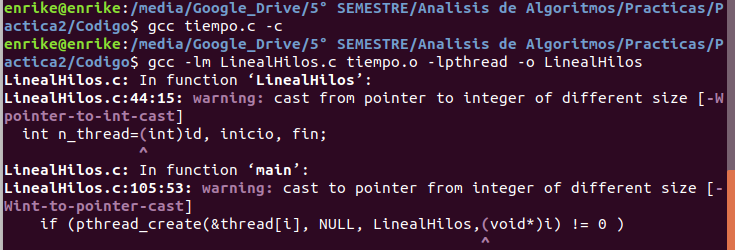
\includegraphics[width=0.8\textwidth]{images/pruebas/warning2.png}
			    	   \caption{Warning al compilar la Búsqueda Lineal con hilos}
			    \end{figure}
			    
			    
	    \begin{figure}[H]
			    	   \centering
			    	   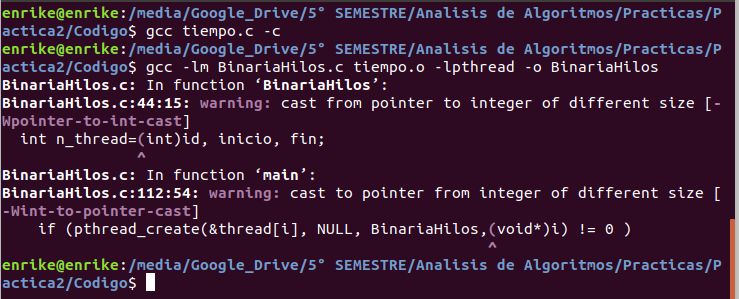
\includegraphics[width=0.8\textwidth]{images/pruebas/warning.png}
			    	   \caption{Warning al compilar la Búsqueda Binaria con hilos}
			    \end{figure}
			    
		Sin embargo, podemos ignorar estas advertencias pues los ejecutables son generados de manera correcta.
		
		\item [\checkmark] En la implementación de la Búsqueda Binaria con hilos, los tiempos de ejecución son mucho mayores a los de la implementación sin hilos.
		
		
	    
	\end{itemize}

\newpage

	% /////////////////////////////////////////////////////////
	%							ANEXOS
	% ////////////////////////////////////////////////////////

	\section{Anexos}

		\subsection{Búsqueda Lineal}
		    \inputminted{c++}{Code/Lineal.c}
		 
		 \subsection{Búsqueda Lineal (Hilos)}
		    \inputminted{c++}{Code/LinealHilos.c}
		    
		 \subsection{Búsqueda Binaria}
		    \inputminted{c++}{Code/Binaria.c}
		 
		 \subsection{Búsqueda Binaria (Hilos)}
		    \inputminted{c++}{Code/BinariaHilos.c}
		 
		 \subsection{Arbin.h}
		    \inputminted{c++}{Code/Arbin.h}
		 
		 \subsection{Árbol de Búsqueda Binaria}
		    \inputminted{c++}{Code/ABB.c}
		 
		 \subsection{Script de Compilación}
		 \inputminted{c++}{Code/script.c}

	% /////////////////////////////////////////////////////////
	%						BIBLIOGRAFIA
	% ////////////////////////////////////////////////////////
	
	\section{Bibliografía}
	
	$[1]$ E. A. Franco Martínez, “Análisis temporal y notación de orden (Algoritmos de búsqueda)” Análisis de Algoritmos, Escuela Superior de Computación, Instituto Politécnico Nacional,
    Ciudad de México, México, Practica02.pdf, Sep. 2018
  
    $[2]$ (2018) WolframAlpha. Accessed september 2018. [Online]. \\Available: http://www.wolframalpha.com/

	\nocite{ref2}
	\bibliography{referencias}
     
\end{document}